\section{OpenACC Object Orientation}

\begin{frame}
	\frametitle{What IS an object?}
    \begin{columns}
        \column{0.5\textwidth}
            \begin{block}{Main aspects of OOP}
                \begin{itemize}
                    \item Objects: data structures containing "base" data and methods
                    \item In memory: contiguous blocks of non-static data + padding
                    \item Principles:
                    \begin{itemize}
                        \item Encapsulation: only class methods should access data
                        \item Inheritance: an object class may be derived from another
                        \item Polymorphism: methods may be redefined in derived classes
                        \item Abstraction: implementation details hidden from user
                    \end{itemize}
                \end{itemize}
            \end{block}
        \column{0.5\textwidth}
        \begin{figure}
            \centering
            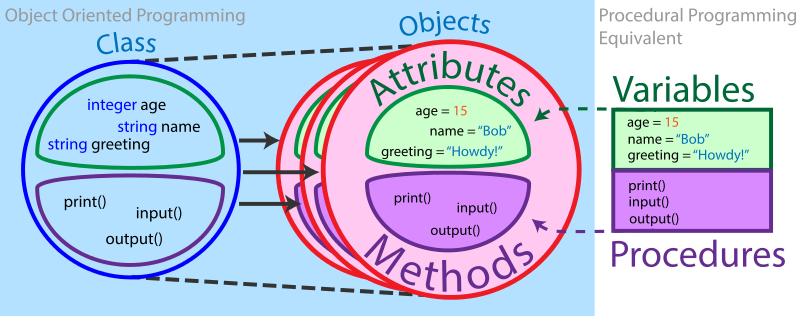
\includegraphics[width=0.95\textwidth]{images/oop.png}
            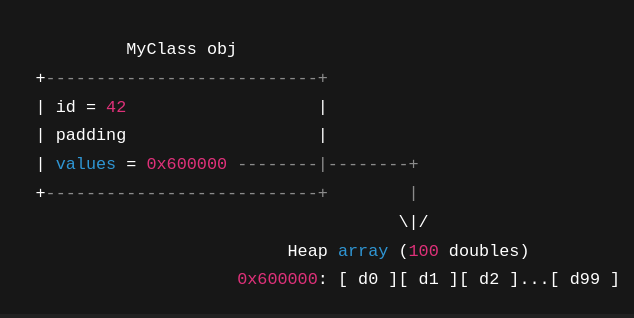
\includegraphics[width=0.95\textwidth]{images/objectLayout.png}
        \end{figure}
    \end{columns}
\end{frame}

\begin{frame}
	\frametitle{Benefits and caveats}
    \begin{columns}
        \column{0.5\textwidth}
            \begin{block}{Pros}
                \begin{itemize}
                    \item Classes are easy to reuse
                    \item Encapsulation ensures data integrity
                    \item Inheritance allows code generalization
                    \item Polymorphism allows flexible code
                    \item Abstraction allows hiding complexity
                    \item Helps to reduce function signature complexity
                    \item Design patterns + OOP can lead to VERY flexible/extensible code
                \end{itemize}
            \end{block}
        \column{0.5\textwidth}
            \begin{alertblock}{Cons}
                \begin{itemize}
                    \item Encapsulation means a LOT of extra methods...
                    \item Padding for alignment leads to memory waste
                    \item Constructor/Destructor methods require careful consideration about object lifetime
                    \item Fortran support for OOP is limited
                    \item Design patterns + OOP can lead to VERY complex code
                    \item CUDA/OpenACC not REALLY designed for OOP!
                \end{itemize}
            \end{alertblock}
    \end{columns}
\end{frame}

\begin{frame}
    \frametitle{Defining a class}
        \begin{block}{C++}
            \lstinputlisting[style=cppstyle]{../oop_disassembly/MyClass.h}
        \end{block}
\end{frame}

\begin{frame}
        \begin{block}{Fortran}
            \lstinputlisting[style=fortranstyle]{../oop_disassembly/mod_myclass.F90}
        \end{block}
\end{frame}

\begin{frame}
    \frametitle{Why OOP is tricky with ACC?}
    \begin{alertblock}{Addressing shenanigans}
        \begin{itemize}
            \item CUDA designed with C in mind: ACC follows that philosophy
            \item Objects are simple "memory blocks", containing data and pointer addresses
            \item Dynamic object data need to be created separately on the device!!!
            \item Arrays of Objects require separate allocation PER OBJECT
            \item Self instantiation on device is "possible", even for AOOs, but tricky
            \item Nested objects are possible, but VERY tricky, especially for AOOs (better with self instantiation)
            \item Fortran has VERY LIMITED support for OOP + ACC: no type-bound procedures on device, no nested AOOs!
            \item Dummy "objects" in Fortran generate copies, and may result in dangling references!
        \end{itemize}
    \end{alertblock}
\end{frame}

\begin{frame}
	\frametitle{Examples}
    \begin{itemize}
        \item Path: \texttt{Lucas/object\_oriented\_acc}
        \item Examples in both C/C++ and Fortran
        \item CMake infra for building provided for all examples
        \item Every example has a \texttt{README.md} with details and suggested exercises
        \item NOTE: some examples are intentionally flawed, as the point is to illustrate pitfalls/limitations
        \item for all examples, run with NSYS to verify memory transfers occuring (vary data sizes to see effects)
    \end{itemize}
\end{frame}

\begin{frame}
    \frametitle{Example 1: Simple objects}
    \begin{itemize}
        \item Objective: show basic object definition and usage with OpenACC
        \item Class contains a scalar and a dynamic array
        \item Fortran case: \texttt{single\_ddt\_with\_allocatable}
        \item C++ case: \texttt{struct\_with\_dynamic\_array}
        \item Key detail: it is NOT sufficient to create the object on device; dynamic data must be created separately!
        \item exercise: on the \texttt{copyout} directive, try reversing the order in which data is copied back to host. What happens?
    \end{itemize}
\end{frame}

\begin{frame}
    \frametitle{Example 2: Arrays of Structures}
    \begin{itemize}
        \item Objective: show how to handle arrays of structures with OpenACC
        \item Not quite an AOO: attributes are public, no need for getters/setters
        \item The \texttt{struct} contains a scalar and a dynamic array
        \item Fortran case: \texttt{multiple\_ddts\_with\_allocatable}
        \item C++ case: \texttt{aos\_with\_dynamic\_arrays}
        \item Key detail: now the driver allocates an array of objects, each object requiring separate allocation of its dynamic data on both host AND device!
        \item NOTE: the Fortran and C++ cases diverge a bit: in the C++ case, the host is created fully, then copied. In Fortran, the allocation loop handles both host and device sides!
        \item Exercise: in either case, the AOO + dynamic array can be substituted by a single 2D array. Try implementing this change and compare performance
    \end{itemize}
\end{frame}

\begin{frame}
    \frametitle{Example 4: Nested AOOs}
    \begin{columns}
        \column{0.5\textwidth}
            \begin{itemize}
                \item Objective: show how to handle nested AOOs with OpenACC, and imposed limitations in Fortran
                \item Russian doll of data: a root AOO where each entry contains another AOO, which in turn contains a dynamic array...
                \item Could easily occur in a FEM code: a 3D element contains an array of 2D faces, each face containing an array of 1D edges, each edge containing an array of nodes, each node containing an array of data...
                \item Allocation sizes per entry need NOT be uniform! Leads to alignment issues and other evils...
            \end{itemize}
        \column{0.5\textwidth}
            \begin{figure}
                \centering
                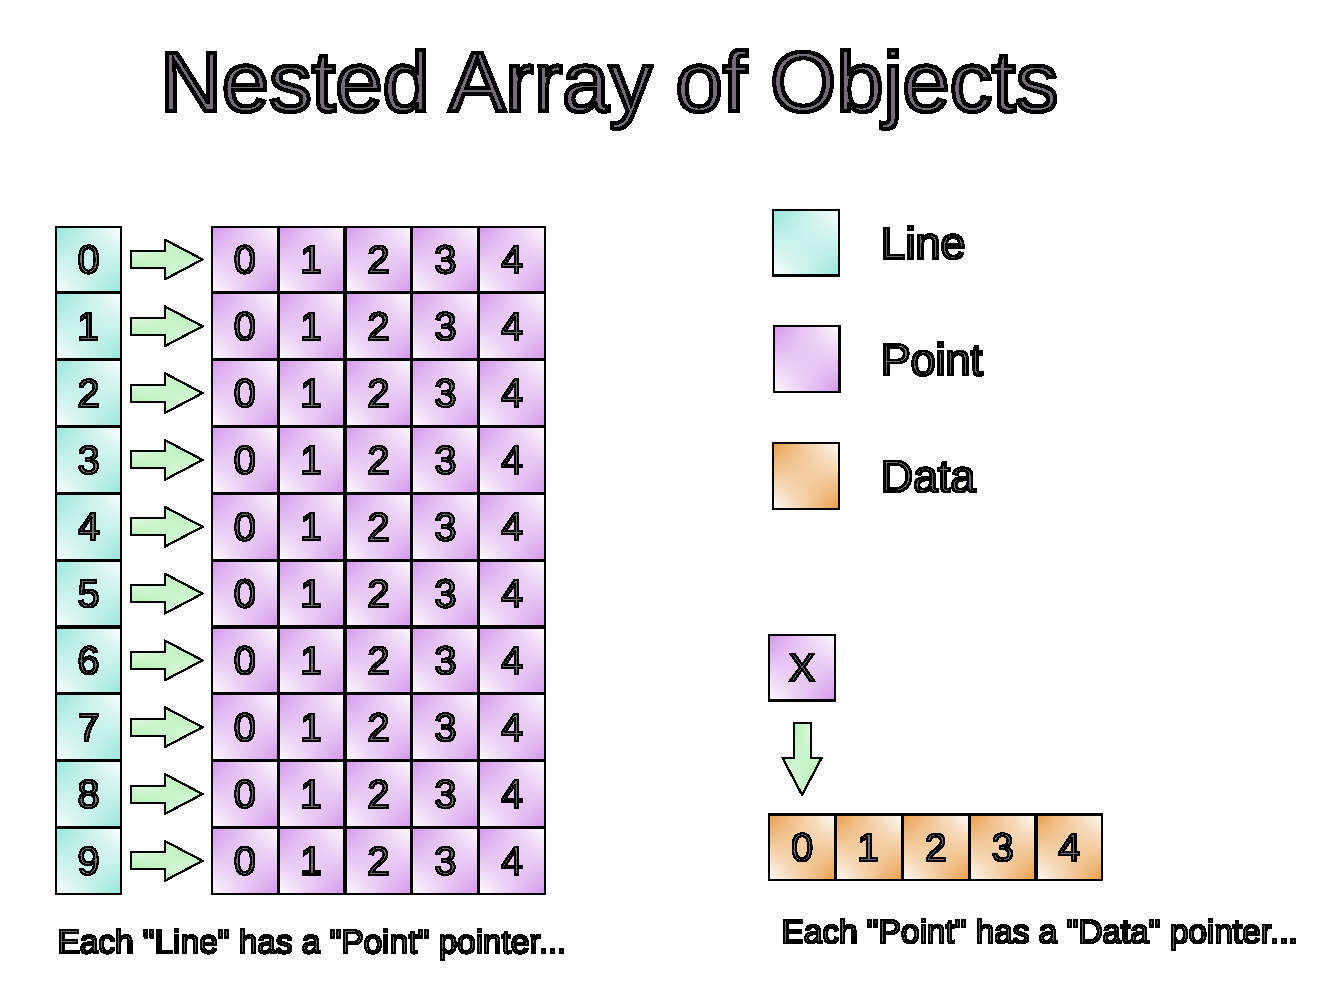
\includegraphics[width=0.95\textwidth]{images/AOO_layout.pdf}
            \end{figure}
    \end{columns}
\end{frame}

\begin{frame}
    \begin{itemize}
        \item Exercise: redo the data structures using flattened arrays (like a traditional C/Fortran code) instead of AOOs. Compare complexity and performance
    \end{itemize}
\end{frame}